\section{Multiplexing}
    Quando la larghezza di banda di un canale trasmissivo è maggiore della larghezza di banda effettivamente necessaria, il canale può essere condivisdo da più trasmissioni contemporaneamente.
    
    \vspace{3mm}
    
    \textbf{Il multiplexing è definito come l'insieme delle tecniche che permettono la trasmissione simultanea di più segnali su un singolo canale di comunicazione.} Utilizzare canali con una larghezza di banda grande per potere trasportare contemporaneamente dati di più canali logici.
    
    \vspace{3mm}
    
    Ad esempio, si ponga il caso di dover spedire dati a 3Mbps su un canale a 10Mbps: in questo caso, sprecheremmo 7Mbps.
    
    \begin{center}
        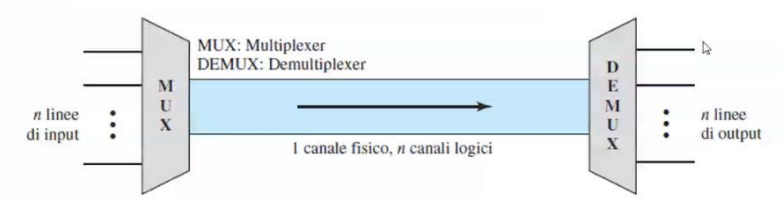
\includegraphics[scale=0.6]{images/Multiplexing.png}
    \end{center}
    
    In un sistema con multiplexing vi è un canale fisico e $n$ linee trasmissive. Per la spedizione occorre aggregare i dati su canali logici e questo lavoro viene svolto dal \textbf{multiplexer} (MUX) che crea un singolo segnale che verrà spedito sul canale fisico; per la ricezione, invece, occorre ridividere i dati aggregati tra i vari canali logici. Il \textbf{demultiplexer} (DEMUX) riconverte il segnale ricevuto nei segnali originali.
    
    \subsection{Tecniche di Multiplexing}
        Esistono tre tecniche generali per implementare il multiplexing.
    
        \begin{itemize}
            \item 
                \textbf{FDM.} E' una tecnica di multiplexing per  segnali analogici. I segnali dei singoli canali logici vengono modulati usando frequenze portanti diverse; i segnali così ottenuti vengono combinati in un singolo segnale composto che può essere trasportato sul collegamento. Le frequenze portanti vengono scelte in modo tale che i segnali modulanti non interferiscano l'uno con l'altro.
                
                \begin{center}
                    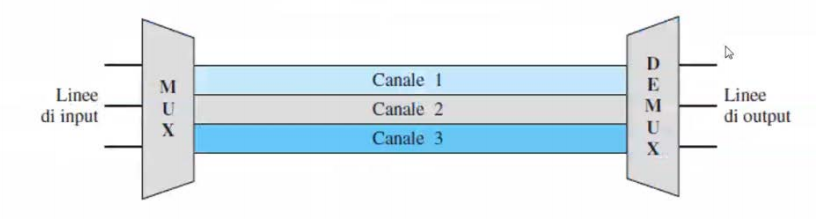
\includegraphics[scale=0.6]{images/FDM.png}
                \end{center}
                
                In fase di \textit{multiplexing}, ogni canale logico genera un segnale sulle stesse frequenze. All'interno del multiplexer questi segnali simili vengono modulati utilizzando segnali portanti di frequenza diversa. I segnali che derivano da ognuna delle modulazioni vengono combinati per creare un singolo segnale composto.
                
                \begin{center}
                    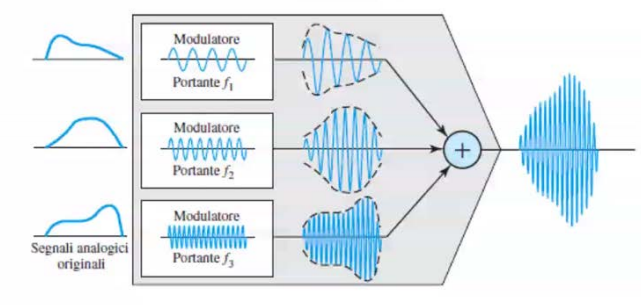
\includegraphics[scale=0.6]{images/FDM_Mult.png}
                \end{center}
                
                In fase di \textit{demultiplexing}, il demultiplexer utilizza una serie di filtri per scomporre il segnale composto ricevuto nei singoli segnali originali. Ciascun segnale viene fatto passare attraverso un demodulatore che supera il segnale che rappresenta i dati originali dal segnale portante usato per modularlo.
            
                \begin{center}
                    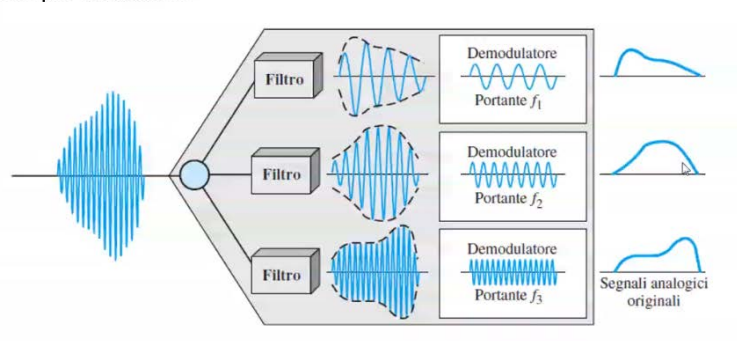
\includegraphics[scale=0.6]{images/FDM_Demult.png}
                \end{center}
            
            \item
                \textbf{WDM.} Tecnica di multiplexing per segnali ottici, utilizza per i cavi in fibra ottica a velocità elevata.
                
                \begin{center}
                    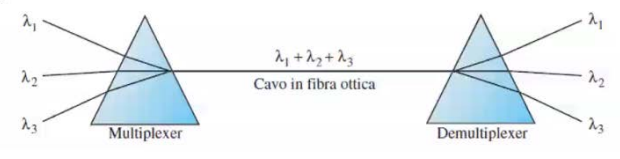
\includegraphics[scale=0.6]{images/WDM.png}
                \end{center}
                
                La modulazione è effettuata sulla lunghezza d'onda del segnale; è una tecnica complessa ma l'idea di base è semplice: si combinano varie sorgenti di luce in un singolo segnale luminoso (multiplexer) o si fa l'esatto opposto (demultiplexer). Le operazioni di raggruppamento e di divisione dei segnal iluminosi possono essere effettuate mediante un prisma, che devia un raggio luminoso in base all'angolo di incidenza e alla frequenza.
             
            \item
                \textbf{TDM.} Progettato per condividere un canale digitale. Invece di condividere una porzione della larghezza di banda, come nel FDM, esso conmdivide il tempo di utilizzo del collegamento. Ogni canale logico occupa un intervallo di tempo in maniera sincrona o statistica.
                
                \begin{center}
                    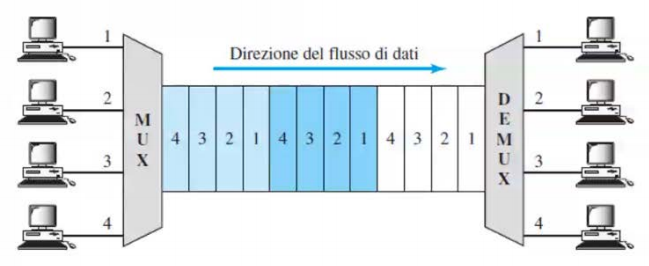
\includegraphics[scale=0.6]{images/TDM.png}
                \end{center}
                
                \begin{itemize}
                    \item 
                        Nel \textbf{TDM sincrono}, l'utilizzo del collegamento fisico viene suddiviso in intervalli di tempo. Il canale viene sfruttato a turno da ogni singolo canale logico. 
                        
                        La grandezza dell'intervallo in sé è un parametro dello schema, che determina il numero di bit che si possono spedire in quell'intervallo. La velocità del collegamento è $n$ volte quella dei canali. 
                        
                        I dati provenienti da ognuno dei canali vengono spediti a turno, seguendo un ordine prestabilito. Gli intervalli sono assegnati staticamente; se un canale non ha dati, l'intervallo viene sprecato.
                    
                        \begin{center}
                            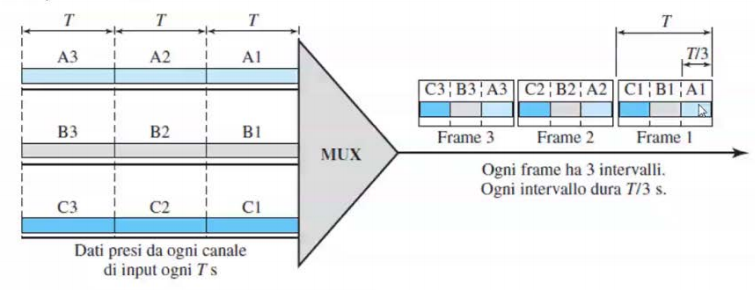
\includegraphics[scale=0.6]{images/TDM_Sincrono.png}
                        \end{center}
                    
                        In particolare, il TDM sincrono può essere \textit{multilivello} (utilizzato quando la velocità delle linee di input sono l'una multiplo dell'altra) e \textit{multiturno} (Alloca più di un turno ad un canale che è più veloce degli altri. Le velocità devono essere tutte multiple di un'unità di base).
                        
                        \vspace{3mm}
                        
                        Il vantaggio del TDM sincrono è la facilità di individuazione dei singoli canali; lo svantaggio è lo spreco di intervalli.
                    
                    \item
                        Nel \textbf{TDM statistico}, \textbf{gli intervalli sono assegnati dinamicamente}. Se un canale non ha dati, l'intervallo viene usato da un altro canale.
                        
                        \vspace{3mm}
                        
                        Il vantaggio del TDM statistico è che usa sempre gli intervalli. Lo svantaggio è che è difficile individuare i singoli canali logici.
                \end{itemize}
        \end{itemize}

        L'implementazione del multiplexing TDM è più complesso di quello FDM. \textbf{La sincronizzazione fra multiplexer e demultiplexer è un problema fondamentale.} Se non sono sincronizzati, l'appartenenza dei bit ai canali logici verrà falsata. 
        
        La soluzione è inserire uno o più \textbf{bit di sincronizzazione} nei frame (anche solo uno, il cui valore si alterna fra 0 e 1).